%%%%%%%%%%%%%%%%%%%%%%%%%%%%%%%%%%%%%%%%%
% Journal Article
% LaTeX Template
% Version 1.4 (15/5/16)
%
% This template has been downloaded from:
% http://www.LaTeXTemplates.com
%
% Original author:
% Frits Wenneker (http://www.howtotex.com) with extensive modifications by
% Vel (vel@LaTeXTemplates.com)
%
% License:
% CC BY-NC-SA 3.0 (http://creativecommons.org/licenses/by-nc-sa/3.0/)
%
%%%%%%%%%%%%%%%%%%%%%%%%%%%%%%%%%%%%%%%%%

%----------------------------------------------------------------------------------------
%	PACKAGES AND OTHER DOCUMENT CONFIGURATIONS
%----------------------------------------------------------------------------------------

\documentclass[twoside,twocolumn]{article}

%\usepackage[showframe, left=2cm, right=2cm, top=32mm, bottom=32mm, columnsep=25pt]{geometry}% http://ctan.org/pkg/geometry
\usepackage{graphicx}% http://ctan.org/pkg/graphicx
\usepackage[left=2cm, right=2cm, top=32mm, bottom=32mm, columnsep=25pt]{geometry}
\usepackage{stfloats}


\makeatletter
\renewcommand{\fnum@figure}{Fig. \thefigure}
\makeatother


\usepackage{blindtext} % Package to generate dummy text throughout this template 

\usepackage[sc]{mathpazo} % Use the Palatino 
\usepackage[T1]{fontenc} % Use 8-bit encoding that has 256 glyphs
\linespread{1.05} % Line spacing - Palatino needs more space between lines
\usepackage{microtype} % Slightly tweak font spacing for aesthetics

\usepackage[english]{babel} % Language hyphenation and typographical rules

%\usepackage[hmarginratio=1:1,top=32mm,columnsep=20pt]{geometry} % Document margins
\usepackage[hang, small,labelfont=bf,up,textfont=it,up]{caption} % Custom captions under/above floats in tables or figures
\usepackage{booktabs} % Horizontal rules in tables
\usepackage{float}
\usepackage{lettrine} % The lettrine is the first enlarged letter at the beginning of the text

\usepackage{enumitem} % Customized lists
\setlist[itemize]{noitemsep} % Make itemize lists more compact
\usepackage{graphicx}

\usepackage{abstract} % Allows abstract customization
\renewcommand{\abstractnamefont}{\normalfont\bfseries} % Set the "Abstract" text to bold
\renewcommand{\abstracttextfont}{\normalfont\small\itshape} % Set the abstract itself to small italic text

\usepackage{titlesec} % Allows customization of titles
\renewcommand\thesection{\Roman{section}} % Roman numerals for the sections
\renewcommand\thesubsection{\roman{subsection}} % roman numerals for subsections
\titleformat{\section}[block]{\large\scshape\centering}{\thesection.}{1em}{} % Change the look of the section titles
\titleformat{\subsection}[block]{\large}{\thesubsection.}{1em}{} % Change the look of the section titles

\usepackage{fancyhdr} % Headers and footers
\pagestyle{fancy} % All pages have headers and footers
\fancyhead{} % Blank out the default header
\fancyfoot{} % Blank out the default footer
\fancyhead[C]{Running title $\bullet$ December 2017 $\bullet$ Aalborg University} % Custom header text
\fancyfoot[RO,LE]{\thepage} % Custom footer text

\usepackage{titling} % Customizing the title section

\usepackage{hyperref} % For hyperlinks in the PDF

\usepackage[utf8]{inputenc}
\usepackage[numbers]{natbib}	
\usepackage[most]{tcolorbox}

\usepackage{subcaption}
%----------------------------------------------------------------------------------------
%	TITLE SECTION
%----------------------------------------------------------------------------------------

\setlength{\droptitle}{-4\baselineskip} % Move the title up

\pretitle{\begin{center}\Huge\bfseries} % Article title formatting
\posttitle{\end{center}} % Article title closing formatting
\title{\huge Prediction of pain duration and intensity from patellofemoral pain maps using deep learning} % Article title
\author{%
\textsc{Birgithe Kleemann Rasmussen, Ignas Kupcikevičius,} \\
\textsc{Linette Helena Poulsen, Mads Kristensen}
 \\[1ex] % Your name
\normalsize Aalborg University \\ % Your institution
% Your email address
%\and % Uncomment if 2 authors are required, duplicate these 4 lines if more
%\textsc{Jane Smith}\thanks{Corresponding author} \\[1ex] % Second author's name
%\normalsize University of Utah \\ % Second author's institution
%\normalsize \href{mailto:jane@smith.com}{jane@smith.com} % Second author's email address
}
\date{December 20, 2017} % Leave empty to omit a date
\renewcommand{\maketitlehookd}{%

\begin{abstract}
\noindent
\textbf{Introduction:} Patellofemoral pain (PFP) syndrome is a musculoskeletal condition that presents as pain behind or around the patella without known structural changes [1]. Partial correlations between perceived size of PFP from pain maps and pain duration along with intensity has been indicated in previous studies [2], however morphology and location of PFP remains unexplored in terms of correlation. Based on the objects detection capabilities of deep learning, convolution methods can be used to detect image-features related to morphology. The aim of this study was to determine the performance of deep learning classification according to pain duration and intensity, based on morphology and location of perceived PFP from pain maps.

\noindent
\textbf{Methods and materials:} PFP drawings were collected on lower extremities body-schema and encoded into three different data representations in respect to morphology of pain and location and a combination of the two. The distribution of the outputs were analyzed and used for defining the classification intervals for pain duration, below 12 months and above 36 months, and pain intensity, below 4 and above 8 on VAS.
Estimation of generalization performance of the models was calculated through 10-fold cross validation during the training.

\noindent
\textbf{Results:} The results during training showed a higher accuracy for pain intensity classification than pain duration classification using morphology-representation. Pain intensity had an accuracy on 65.04\% (SD: $10.83\%$) and pain duration had an accuracy on 59.51\% (SD: $11.20\%$).
\noindent
Furthermore, the combined-representation performed with the highest accuracy on 65.14\% (SD: $12.87\%$). The location and morphology-representation scored 63.33\% (SD: $1.67$) and 65.04\% (SD: $10.83\%$), respectively, based on pain intensity. 

\noindent
\textbf{Discussion:} Despite pain intensity being defined as multidimensional and subjective, the performance accuracy were higher than that of pain duration. The results may indicate that a combination of the morphology and the location of the pain had a higher classification performance in relation to pain duration or intensity. Currently, it is unclear if deep learning methods may be a suitable approach for classifying PFPS to work as support in clinical settings, to which further investigation is necessary. Improvements could be found when more data become available to better reflect generalization patterns in PFP drawings.
\end{abstract}
}

%----------------------------------------------------------------------------------------
%\usepackage[left=2cm, right=2cm, top=32mm, bottom=32mm, columnsep=25pt]{geometry}
\begin{document}

% Print the title
\maketitle

%----------------------------------------------------------------------------------------
%	ARTICLE CONTENTS
%----------------------------------------------------------------------------------------

\section{Introduction}
Patellofemoral pain syndrome (PFPS) is a painful musculoskeletal condition that is presented as pain behind or around the patella \citep{Maclachlan2017, Smith2015}. PFPS affects 6-7 \% of adolescents, of whom two thirds are highly physically active \citep{Rathleff2015}. Additionally the prevalence is more than twice as high for females than males \citep{Rathleff2015, Petersen2013}.
PFPS may be present over a longer period of time where a high number of individuals experience a recurrent or chronic pain \citep{Witvrouw2014} and may also lead to osteoarthritis \citep{Petersen2013, Crossley2016}.

\noindent
Patellofemoral pain (PFP) is often described as diffuse knee pain, that can be hard for individuals to explain and localize \citep{Witvrouw2014}. Despite the fact that individuals feel pain in the knee, there is no structural changes in the knee such as significant chondral damage or increased Q-angle. Because of this there is no definitive clinical test to diagnose PFPS and it is thereby often diagnosed based on exclusion criterias \citep{Petersen2013} to which PFPS is also described as an orthopaedic enigma, and is one of the most challenging pathologies to manage \citep{Dye2001}.
To assist diagnosis of PFPS, pain maps may be used as a helpful tool for the individuals to communicate their pain by drawing pain areas on a body outline \citep{Boudreau2016}. 

\noindent
A study by \citeauthor{Boudreau2017} indicates through the use of pain maps that it is possible to find a correlation between the size of the pain and the pain duration as well as intensity for individuals with PFP longer than five years.\citep{Boudreau2017} However, it is unknown whether the morphology and locations of the pain have an influence on the pain duration and intensity. 
It is assumed that relation between pain maps and pain duration or intensity is nonlinear, because the perceived PFP is subjective and is considered as multidimensional \citep{Dansie2013}. To investigate the nonlinear relation, deep learning is used, which is a method that has not been found used in this context before.

\noindent
The goals of this project is to explore how accurate a deep learning model can classify pain maps according to pain duration and intensity by using a limited dataset. The pain maps are encoded into multiple data representations to investigate whether morphology and location have an influence on pain duration or intensity. Because of the imbalance in prevalence between females and males, the gender is included as a feature in the deep learning model. \newline

\noindent
The aim of this study is to explore classification performance of a deep learning model, using PFP pain maps and gender as input to classify either pain duration or intensity.


\begin{center}
\textit{It is hypothesized that a deep learning model that uses pain maps and gender as input parameter has a higher performance when classifying according to pain duration than pain intensity.}
\end{center}

\noindent
The secondary aim is to investigate if multiple pain map representations, which reflect the morphology and location of the pain, affect the deep learning model classification performance.                                                    
\begin{center}
\textit{It is hypothesized that different data represen-\newline tations of pain maps, reflecting morphology and location of pain, affect the performance
accuracy of a deep learning model when classifying according to pain duration or intensity.
}
\end{center}



%------------------------------------------------

\section{Methods}
\textbf{Pain maps} \newline
Data used in this study were collected beforehand from an on-going clinical trial (FOXH) which is conducted in collaboration with Danish and Australian universities. The pain maps were drawn by individuals with PFPS through the use of an application, Navigate Pain, in a clinical setting. \newline
\noindent
Navigate Pain is a software application that is used to visualise the location, morphology and spatial distribution of pain from individuals to healthcare personnel. The application permits individuals to draw their pain with different colors and line thickness onto a body outline, an example is shown in fig. \ref{fig:twoPainmaps}. Navigate Pain android was developed at Aalborg University.\citep{Solutions2015}

\begin{figure}[H]
\centering
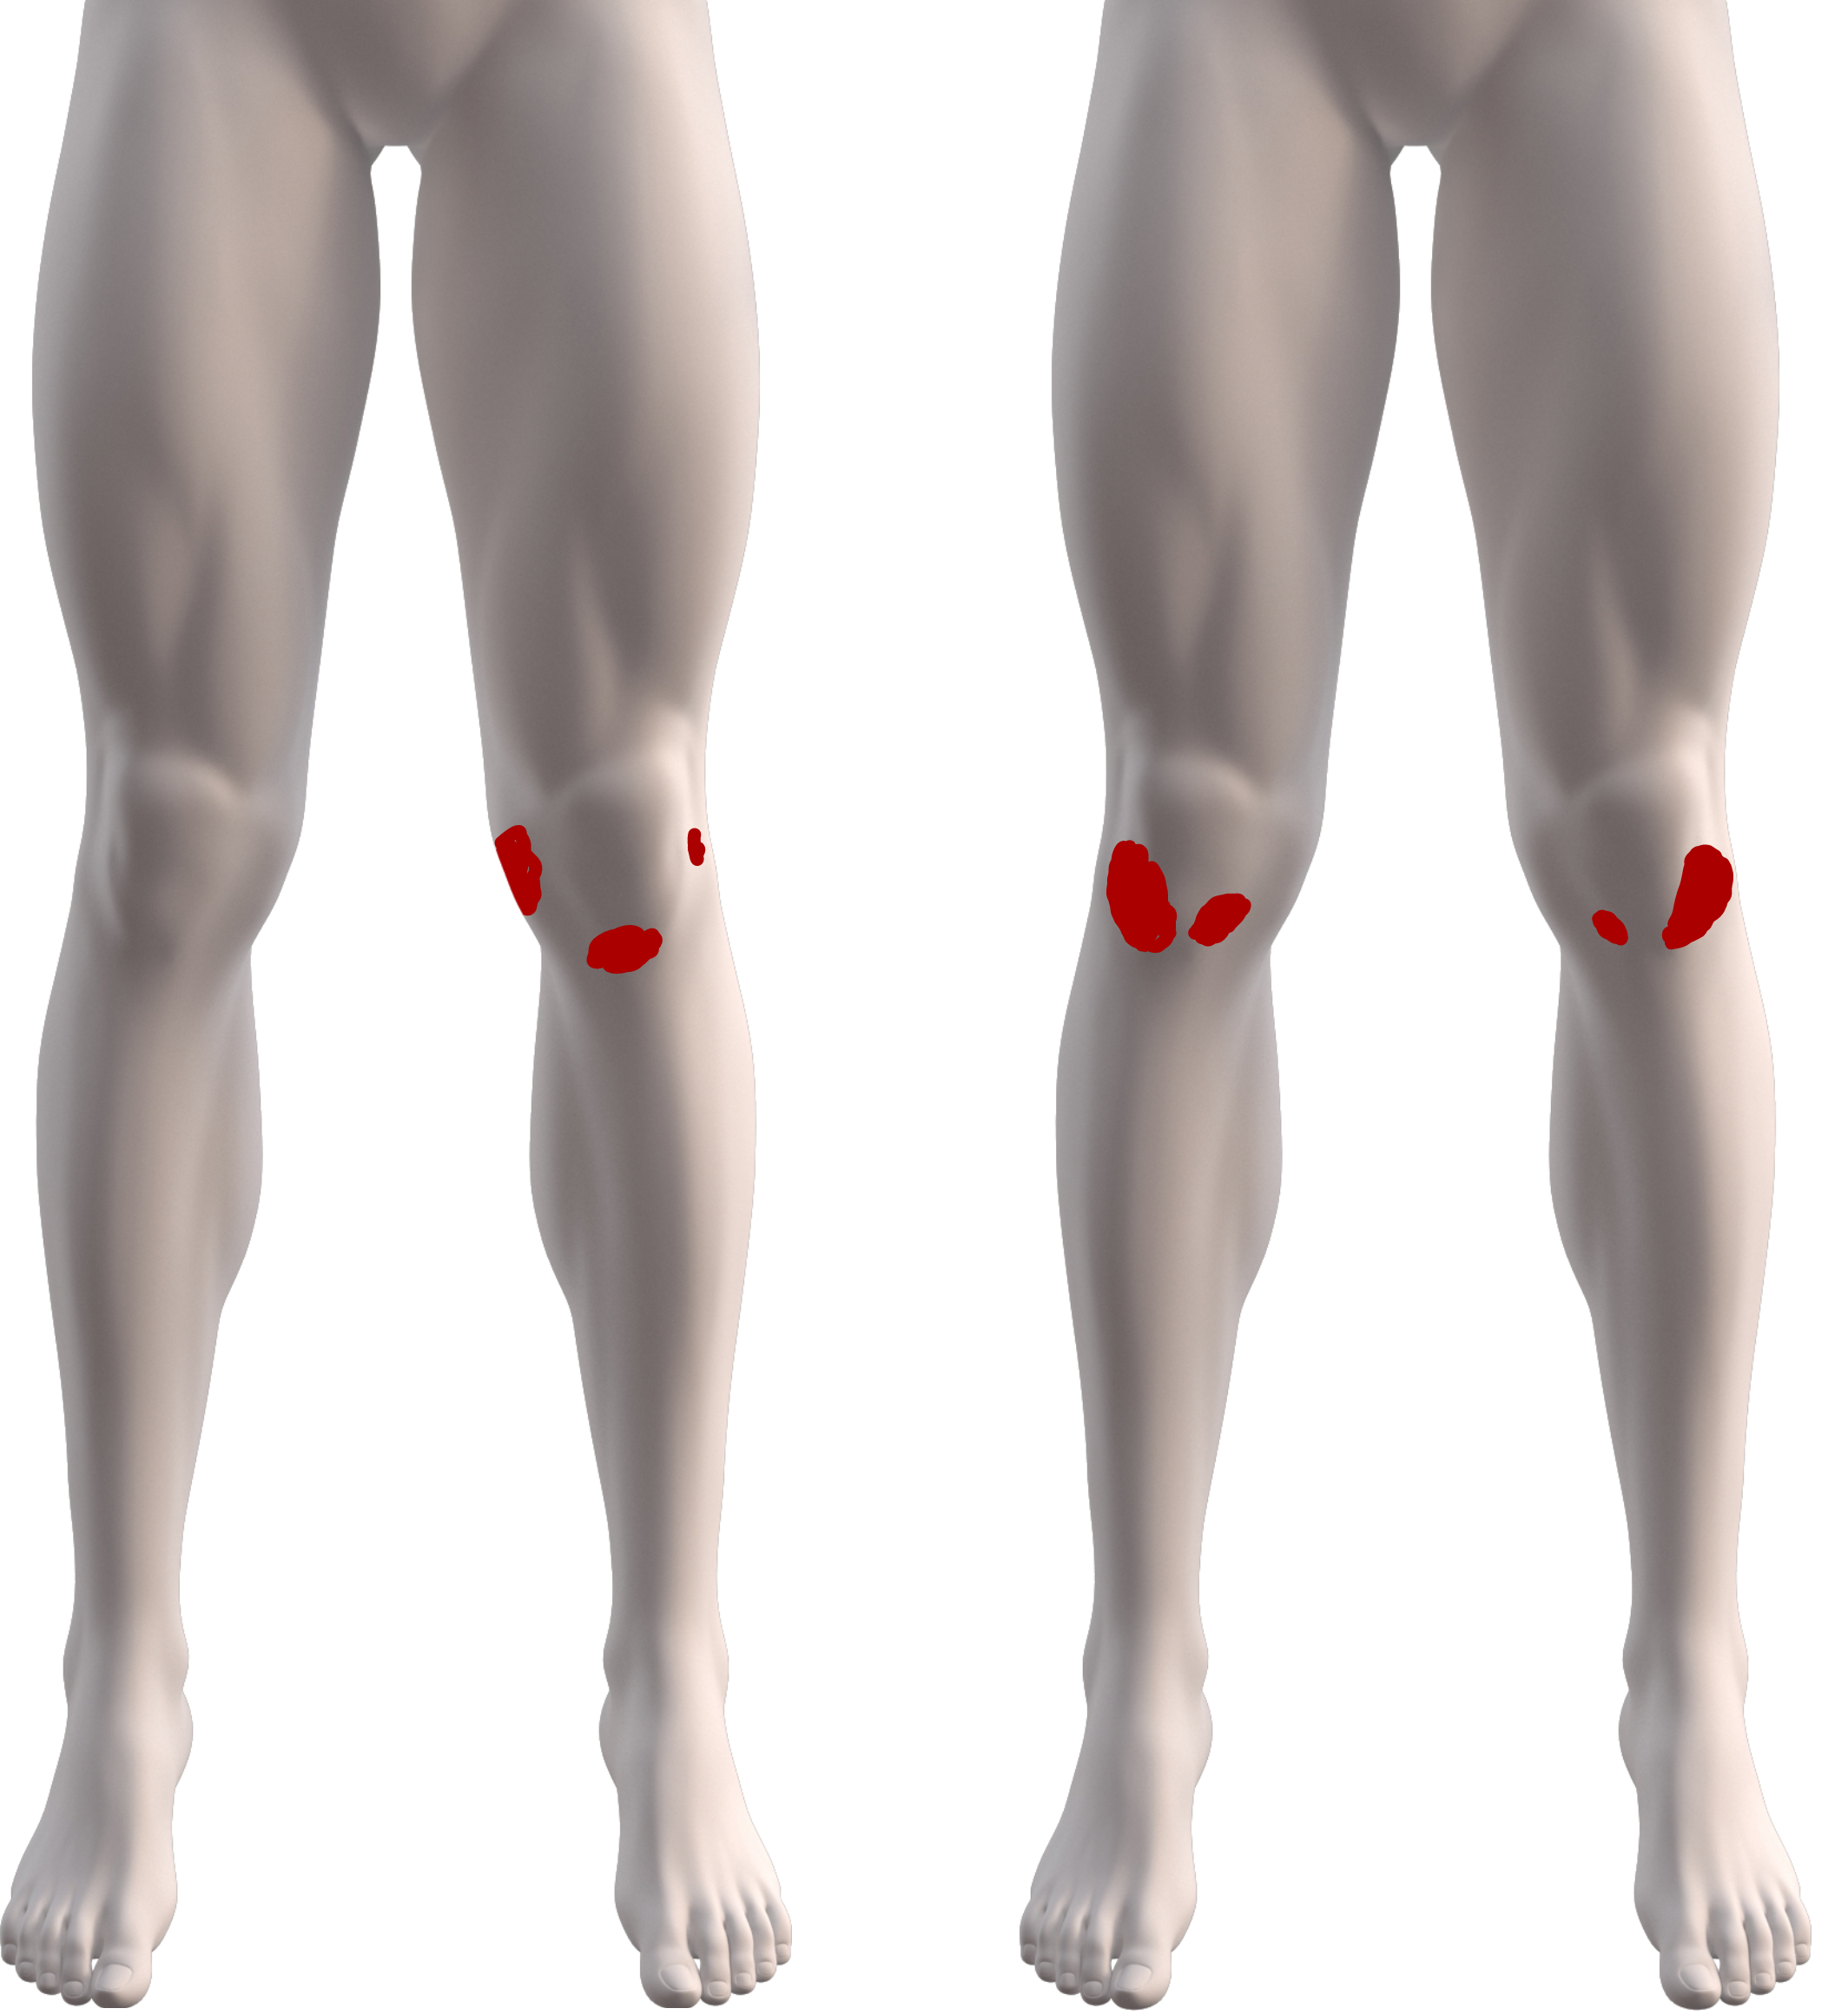
\includegraphics[width=0.35\textwidth]{Figures/twoPainmaps}
\caption{Pain maps from individuals with uni- and bilateral PFP. The red markings indicate the area of pain perceived by the individuals.}
\label{fig:twoPainmaps}
\end{figure}

\noindent
The total number of pain maps available was 217, but only 205 pain maps with associated gender and pain duration, and 197 pain maps with associated gender and pain intensity was available.\\

\noindent
\textbf{Preprocessing} \newline
\noindent
The pain maps were processed in MatLab, where the images were resized, since they were collected at different resolutions (screen sizes) and cropped to only include the knees. To create more pain maps is a split body approach used, where pain maps are divided into two knees. Furthermore, pain was mirrored to represent pain on right knees to minimize the variance in the images. By using split body approach it was assumable that the pain duration and pain intensity were identical for both knees if PFP was bilateral. The total number of pain maps with gender and pain duration was 333, and pain maps with gender and pain intensity was 319. \\

\noindent
\textbf{Morphology-representation} \newline
\noindent
The original pain maps reflect the morphology of the pain, and do not require further processing than converting the pain maps to a matrix including gender and the output, pain duration or pain intensity.\\


\noindent
\textbf{Pain location} \newline
\noindent
The knees are divided into regions based on the underlying anatomical structures, which may have a correlation to pain duration or pain intensity.
The locations are divided into 20 regions, which are inspired by Photographic Knee Pain Map (PKPM). The divisions are designed to categorise location of knee pain for diagnostic and research purposes. PKPM represent both knees that makes it possible to identify unilateral and bilateral pain.\citep{Elson2010} The knee regions are illustrated in fig. \ref{fig:atlas}.

\begin{figure} [H] 
\centering
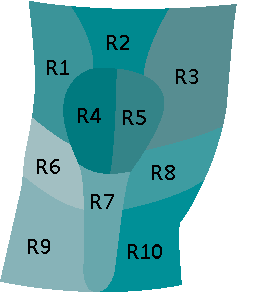
\includegraphics[width=0.35\textwidth]{Figures/atlas}
\caption{The regions of the left (L1-L10) and right (R1-R10) knees, where each knee is split into ten regions.}
\label{fig:atlas}
\end{figure}

\noindent 
There are ten regions on each knee, where region 1 and 3 represent the superior lateral and superior medial areas for patella. Region 2 refers to quadriceps tendon. The patella is divided into lateral and medial regions, which are region 4 and 5. Region 6 and 8 are lateral and medial joint line areas. Patella tendor is region 7 and the two last regions, 9 and 10, are tibia lateral and medial.\citep{Elson2010}\\


\noindent
\textbf{Location-representation} \newline
\noindent
To investigate whether the location alone have a correlation to the outputs, a simplified representation of the pain maps was created. The location of the pain was reflected by the use of the defined knee regions (fig. \ref{fig:atlas}), where each region represented a value of 0 (not active) or 1 (active) in a vector.  The values were defined by using a threshold to determine whether a region was considered active in relation the amount of pain. A threshold was required to increase the confidence of an active pain region by avoiding minimal contributions e.g. small pain areas in the associated regions. Simultaneously the threshold should not be too large so that pain areas was excluded. The threshold was decided based on an analysis on five random pain maps, where threshold values of 0, 5, 10 and 15\% was compared. The threshold represent which minimal percentage of pain should be present in a specific region before it is considered active. Based on the analysis a 5\% threshold was chosen. As a result for adding the threshold value the number of pain maps with pain duration decrease to 316, and number of pain maps with pain intensity decrease to 302.  \newline

\noindent
\textbf{Combined-representation} \newline
\noindent
A combination of morphology and location of the pain is created based on components from morphology- and location-representations. The original pain maps are superimposed on the regions, which result in pain pixels reflecting the location with a number from 1 to 10. Before using the representation as input, one-hot encoding approach was used, which made it possible to separate categorical data into binary data [46]. This means that the 20 values for each knee region do not have a correlation when analysed in the deep learning model. The number of pain maps with pain duration was 331, and number of pain maps with pain intensity was 317. The number of pain maps increased according to the location-representation, because no threshold was applied in this data-representation. 



\noindent
\textbf{Linear regressions} \newline
\noindent
It was assumed that the data was nonlinear, because PFP is subjective and multidimensional. To verify this assumption of nonlinearity, linear regression on simple features reflecting the size of the pain was investigated. This decision was based on the phenomenon central sensitization that may result in widespread, to which this might be reflected in the number of pain pixels and active pain regions. 
Additionally, is a linear correlation according to the pain intensity investigated. The linear regression is shown in fig. \ref{fig:correlations}.



\begin{figure*} [b!]
\begin{tcolorbox}[colframe=black!30!black, colback=white]
\hfill
\begin{subfigure}[r]{0.5\textwidth}
    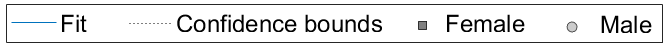
\includegraphics[width=\textwidth]{Figures/legend}
  \end{subfigure}
  \vskip\baselineskip
  \hspace{-5mm}
  \begin{subfigure}[b]{0.51\textwidth}
    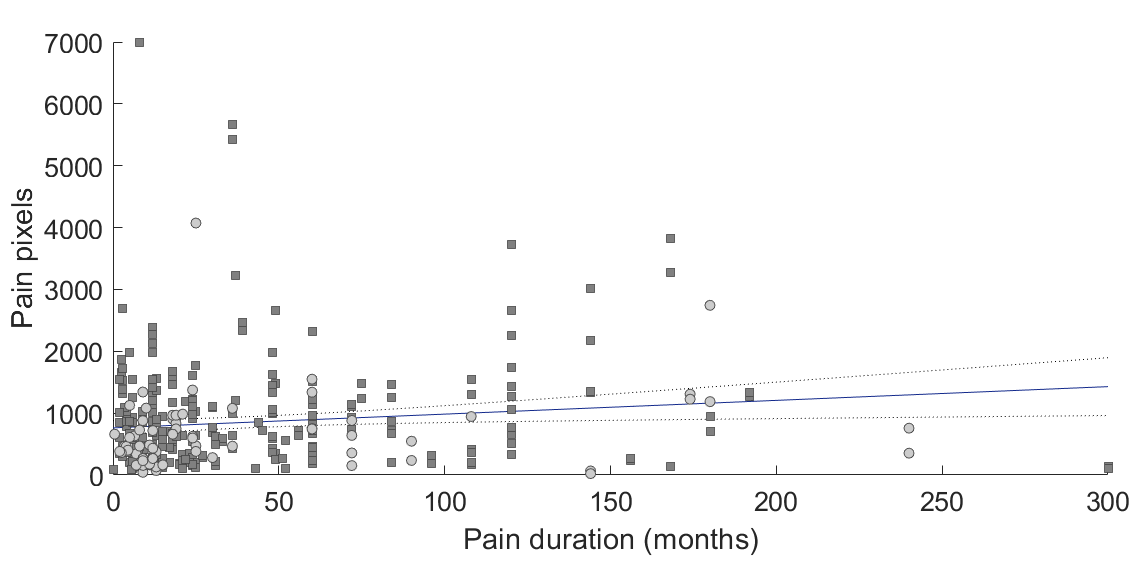
\includegraphics[width=\textwidth]{Figures/durapixel}
    \caption{ }
    \label{fig:1}
  \end{subfigure}
  \hfill
    \hspace{2mm}
  \begin{subfigure}[b]{0.51\textwidth}
    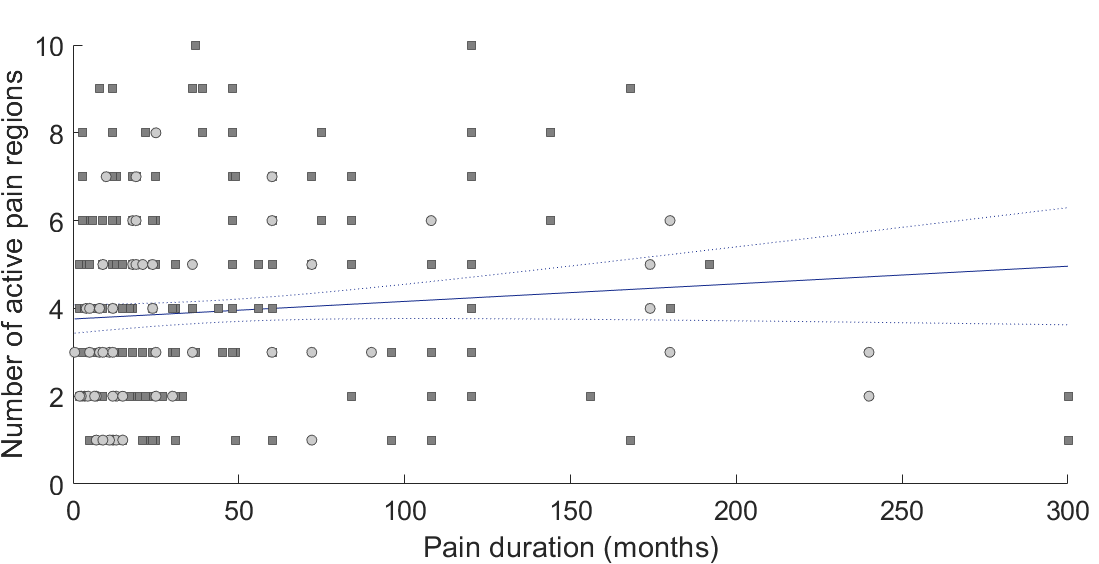
\includegraphics[width=\textwidth]{Figures/duraregion}
       \caption{ }
    \label{fig:2}
  \end{subfigure}
    \vskip\baselineskip
    \hspace{-5mm}
  \begin{subfigure}[b]{0.51\textwidth}
    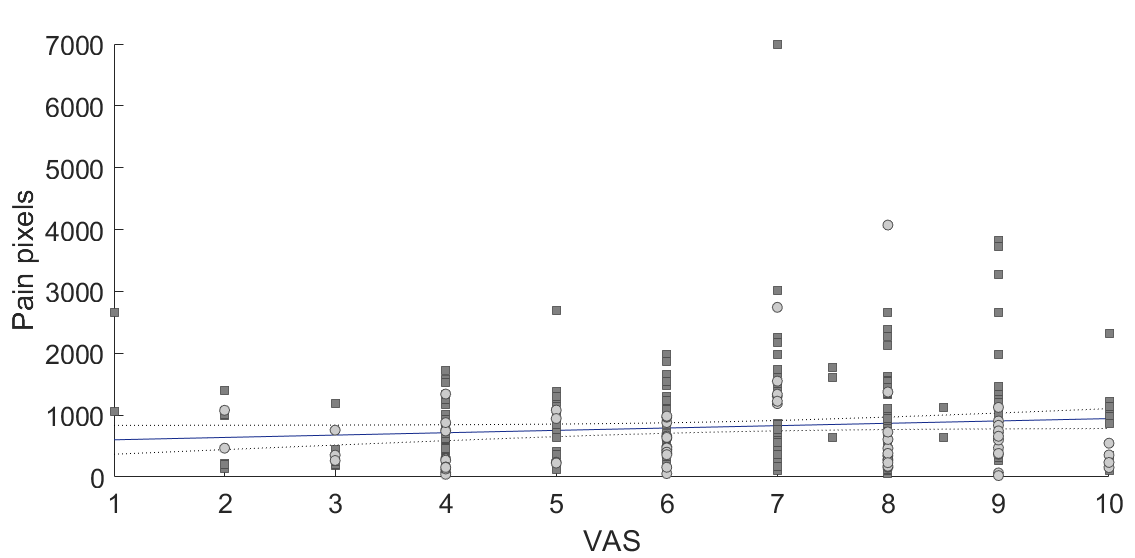
\includegraphics[width=\textwidth]{Figures/vaspixel}
    \caption{}
    \label{fig:3}
  \end{subfigure}
  \hfill
  \hspace{2mm}
  \begin{subfigure}[b]{0.51\textwidth}
    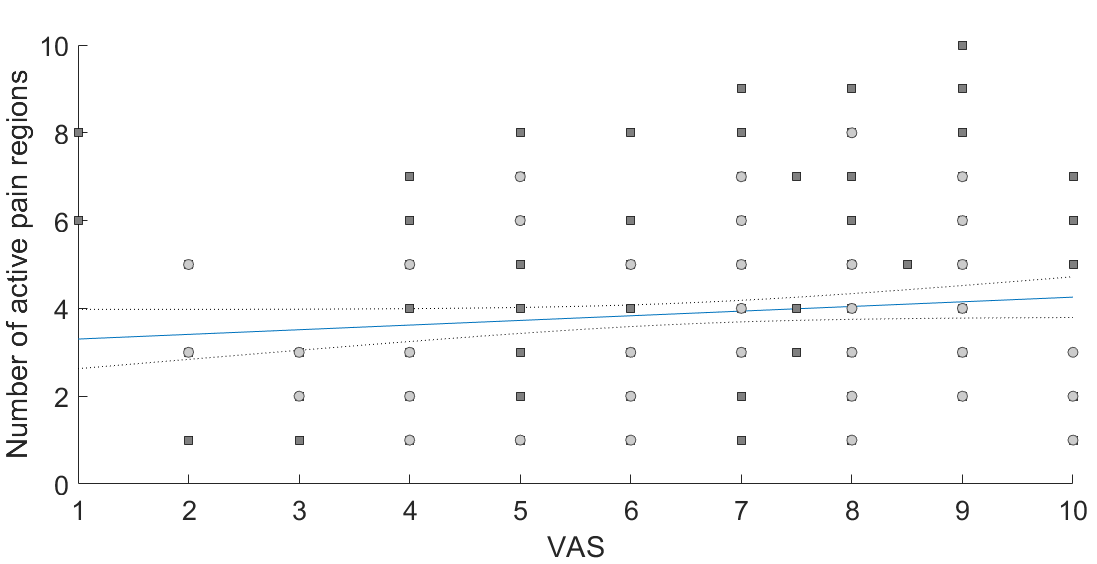
\includegraphics[width=\textwidth]{Figures/vasregion}
       \caption{ }
    \label{fig:4}
  \end{subfigure}  
  \caption{Linear correlations of pain pixels and pain duration (a), active pain regions and pain duration (b), pain pixels and pain intensity indicated in VAS (c), and active pain regions and pain intensity indicated in VAS (d).}
  \label{fig:correlations}
\end{tcolorbox}
\end{figure*}

\noindent
Based on the four linear regression models, it was shown that single features, number of pain pixels or number of active pain regions, did not have a clear linear correlation with the outputs, pain duration or intensity. Hence a deep learning model may find patterns in the pain maps according morphology or location of pain in relation to either pain duration or intensity. \newpage

\noindent
\textbf{Deep learning models}\newline
\noindent
Deep learning models were developed on a computer with 4x ‘‘Intel® Core™ i7‘‘ CPUs and one single GPU of type "Geforce GTX 970M", using the programming language Python v3.6.3. Libraries used was Keras with a TensorFlow backend. \newline
\noindent
Multiple deep learning models suitable to the three data representation were created. The models used supervised learning, which is defined as a network learning to classify a given input corresponding to a specific output \citep{Goodfellow2016}. The models classify the input, pain maps and gender, in relation to the determined outputs, pain duration or pain intensity.\newline
\noindent
Two of the models, which managed the morphology-, and the combined morphology and location-representations, were developed using the same model architecture consisting of convolutional- followed by pooling layers and fully connected layers. Convolutional were used because it’s highly classification in images that automatically learn a complex pattern by extracting visual features from the pixel-level content \citep{Acquarelli2017,LeCun1998}. The combination of convolutional and pooling layers performed feature extraction while the classification was made by fully connected layers. \newline
\noindent
The model that classified the location should not process morphology, thus a convolutional layer was not necessary, and thereby only contained fully connected layers. \\


\noindent
\textbf{Optimization of models}\newline
\noindent
Optimization of the three model were done using a validation subset, whereto graphs plotting validation accuracy and loss were compared with training accuracy and loss. This was used to estimate the optimal number of epochs to reduce overfitting the model to the training subset. Further optimization were done using manual search on hyperparameters, from which improvements were based on an average accuracy, sensitivity and specificity gained from 10-fold cross validation.  

%\begin{figure*} [b!]
%\begin{tcolorbox}[colframe=black!30!black, colback=white]
%\centering
%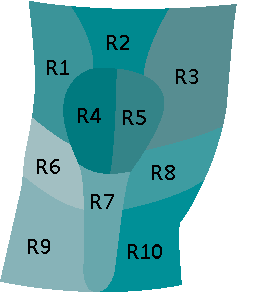
\includegraphics[width=0.2\textwidth]{Figures/atlas}
%\caption{SÅDAN LAVER VI EN BOXER MED ET BILLED}
%\label{fig:atlas1}
%\end{tcolorbox}
%\end{figure*}



%\begin{figure*} [b!]
%\begin{tcolorbox}[colframe=black!30!black, colback=white]
%  \begin{subfigure}[b]{0.45\textwidth}
%    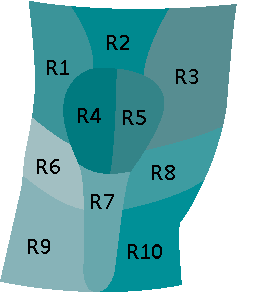
\includegraphics[width=\textwidth]{Figures/atlas}
%    \caption{FUCK JA}
%    \label{fig:f11}
%  \end{subfigure}
%  \hfill
%  \begin{subfigure}[b]{0.45\textwidth}
%    \includegraphics[width=\textwidth]{Figures/twopainmaps}
%    \caption{FUCK NEJ}
%    \label{fig:f22}
%  \end{subfigure}
%  \caption{SÅDAN SÆTTER VI TO BILLEDER I EN}
%\end{tcolorbox}
%\end{figure*}




%------------------------------------------------

\section{Results}

\begin{figure*} [b!]
\begin{tcolorbox}[colframe=black!30!black, colback=white]
\hfill
\begin{subfigure}[r]{0.5\textwidth}
    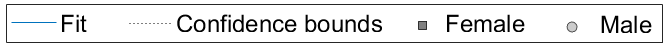
\includegraphics[width=\textwidth]{Figures/legend}
  \end{subfigure}
  \vskip\baselineskip
  \hspace{-5mm}
  \begin{subfigure}[b]{0.51\textwidth}
    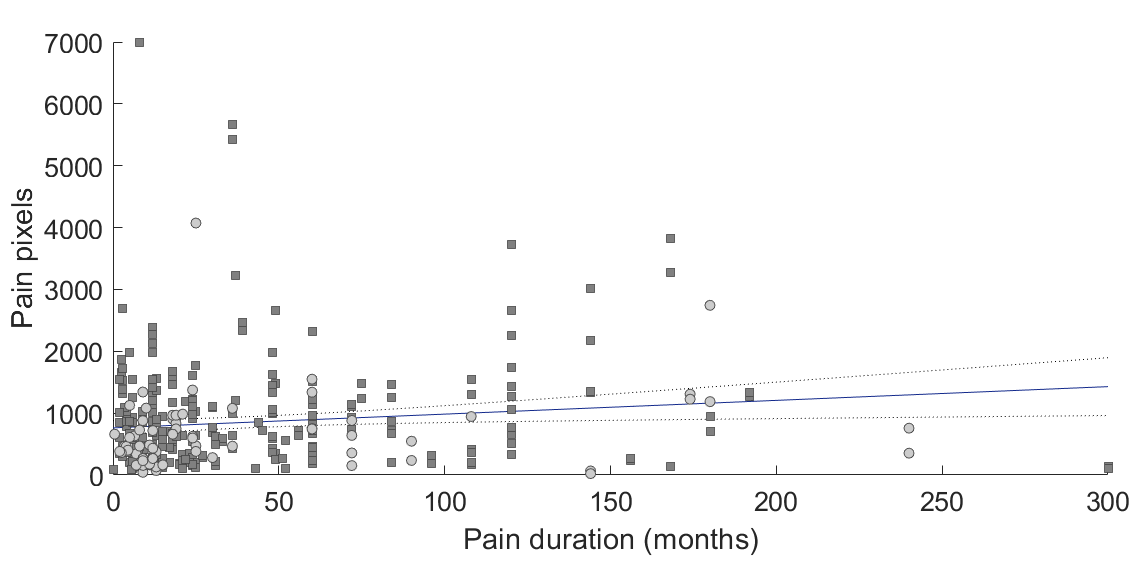
\includegraphics[width=\textwidth]{Figures/durapixel}
    \caption{ }
    \label{fig:1}
  \end{subfigure}
  \hfill
    \hspace{2mm}
  \begin{subfigure}[b]{0.51\textwidth}
    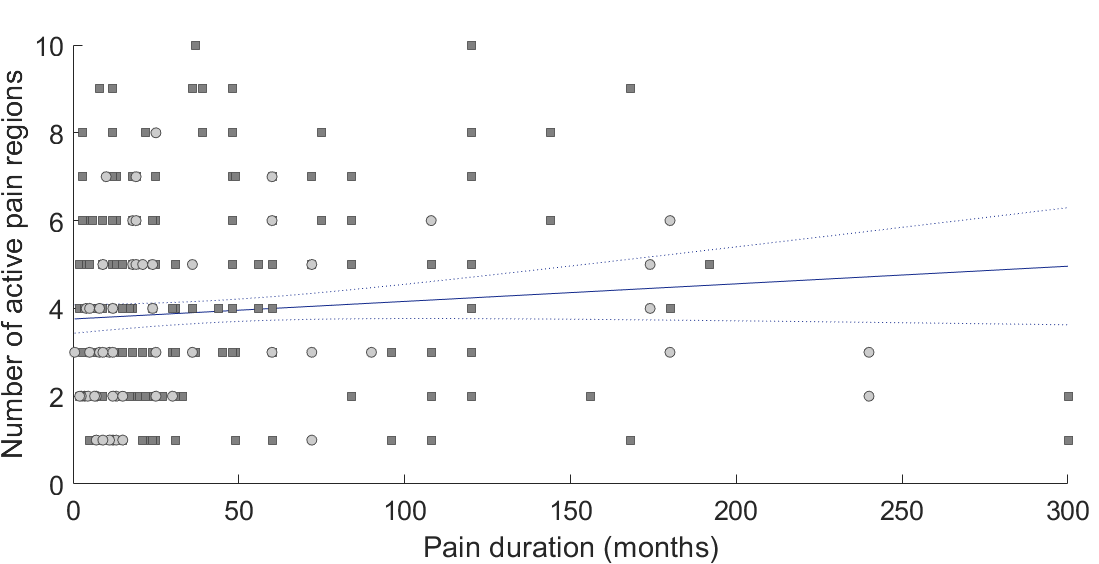
\includegraphics[width=\textwidth]{Figures/duraregion}
       \caption{ }
    \label{fig:2}
  \end{subfigure}
    \vskip\baselineskip
    \hspace{-5mm}
  \begin{subfigure}[b]{0.51\textwidth}
    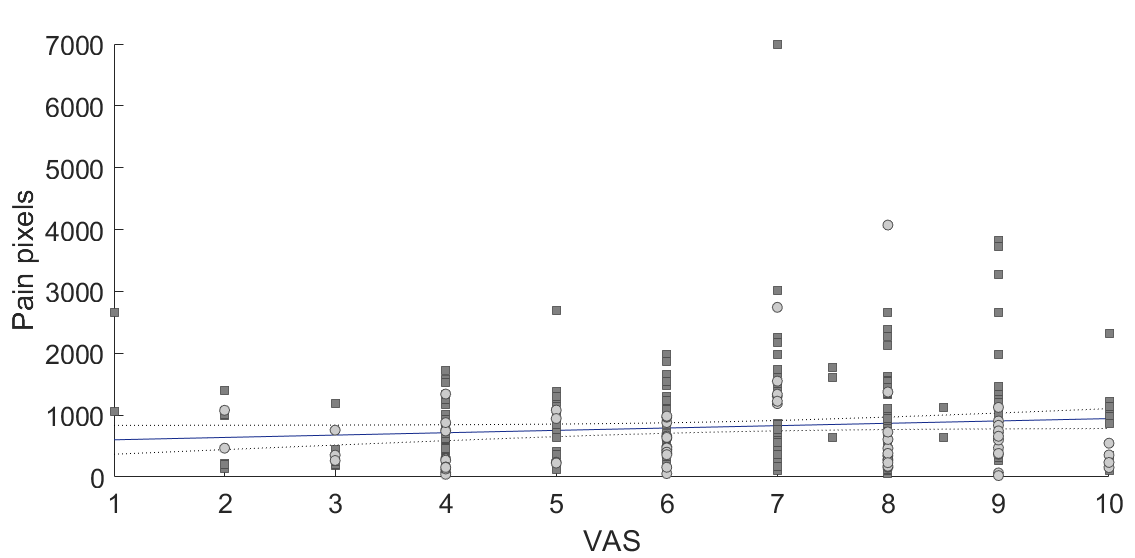
\includegraphics[width=\textwidth]{Figures/vaspixel}
    \caption{}
    \label{fig:3}
  \end{subfigure}
  \hfill
  \hspace{2mm}
  \begin{subfigure}[b]{0.51\textwidth}
    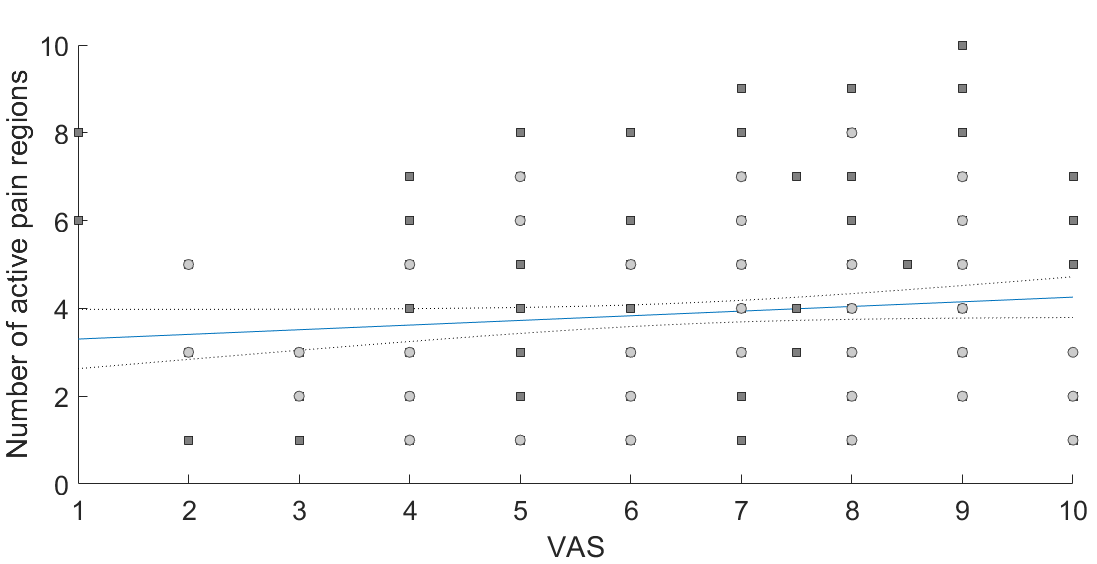
\includegraphics[width=\textwidth]{Figures/vasregion}
       \caption{ }
    \label{fig:4}
  \end{subfigure}  
  \caption{Linear correlations of pain pixels and pain duration (a), active pain regions and pain duration (b), pain pixels and pain intensity indicated in VAS (c), and active pain regions and pain intensity indicated in VAS (d).}
  \label{fig:correlations}
\end{tcolorbox}
\end{figure*}

This section visualize the result from the linear regressions, and performance of the deep learning models using multiple pain maps representation, and different outputs. 
\vspace{-0.3cm}

\subsection*{Linear correlations}
The linear regression between simple features, number of pain pixels or active pain regions, and outputs, pain duration or pain intensity, resulted in the plots shown in fig. \ref{fig:correlations}. The $R^2$-values support the nonlinearity, shown in the plots, where correlation fig. \ref{fig:1} resulted in a $R^2 = 0.018$, fig. \ref{fig:2} resulted in $R^2 = 0.008$, fig. \ref{fig:3} resulted in $R^2 = 0.011$ and fig. \ref{fig:4} resulted in $R^2 = 0.011$. 


\begin{table*}[b!]
\centering
\begin{tabular}{@{}llll@{}}
\toprule
\multicolumn{4}{c}{\hspace{2.3cm} Avg. accuracy (\%) \hspace{1cm} Avg. sensitivity (\%) \hspace{1cm} Avg. specificity (\%) \hspace{1cm}                }                                                                                                                                                                         \\ \midrule
\multicolumn{4}{c}{Morphology-representation} \\ \midrule
Pain duration  & \hspace{0.7cm}\begin{tabular}[c]{@{}l@{}}69.44\% \end{tabular} & \hspace{2.6cm} \begin{tabular}[c]{@{}l@{}}69.23\%\end{tabular} & \hspace{2.7cm} \begin{tabular}[c]{@{}l@{}} 69.57\%\end{tabular} \\ %\midrule
Pain intensity & \hspace{0.6cm} \begin{tabular}[c]{@{}l@{}}60.00\% \end{tabular}  & \hspace{2.7cm}\begin{tabular}[c]{@{}l@{}}40.00\% \end{tabular}  & \hspace{2.7cm} \begin{tabular}[c]{@{}l@{}}70.00\%\end{tabular}   \\ \midrule
\multicolumn{4}{c}{Location-representation}                                                                                                                                                                             \\ \midrule
Pain duration  & \hspace{0.6cm} \begin{tabular}[c]{@{}l@{}}35.29\%\end{tabular}  & \hspace{2.6cm} \begin{tabular}[c]{@{}l@{}}0.00\% \end{tabular}  & \hspace{2.7cm} \begin{tabular}[c]{@{}l@{}}35.29\%\end{tabular}  \\ %\midrule 
Pain intensity & \hspace{0.6cm} \begin{tabular}[c]{@{}l@{}}60.71\% \end{tabular}   & \hspace{2.6cm} \begin{tabular}[c]{@{}l@{}}0.00\% \end{tabular}   & \hspace{2.7cm} \begin{tabular}[c]{@{}l@{}}60.71\%\end{tabular}  \\ \midrule
\multicolumn{4}{c}{Combined-representation}                                                                                                                                                              \\ \midrule
Pain duration  & \hspace{0.6cm} \begin{tabular}[c]{@{}l@{}}55.56\% \end{tabular}                                                                   & \hspace{2.6cm} \begin{tabular}[c]{@{}l@{}}61.11\%\end{tabular}                                                                & \hspace{2.7cm} \begin{tabular}[c]{@{}l@{}}50.00\%\end{tabular}                                                                                                                                \\% \midrule
Pain intensity & \hspace{0.6cm} \begin{tabular}[c]{@{}l@{}}73.33\% \end{tabular}
&\hspace{2.6cm} \begin{tabular}[c]{@{}l@{}} 0.00\%\end{tabular}                                                               
& \hspace{2.7cm} \begin{tabular}[c]{@{}l@{}} 73.33\%\end{tabular}                                                               
 \\ \bottomrule
\end{tabular}
\caption{Generalization performance of the models, which use the morphology-, location- and combined-representation when classifying according to pain duration or pain intensity.}
\label{tab:performance}
\end{table*}


\begin{figure*} [b!]
\begin{tcolorbox}[colframe=black!30!black, colback=white]
    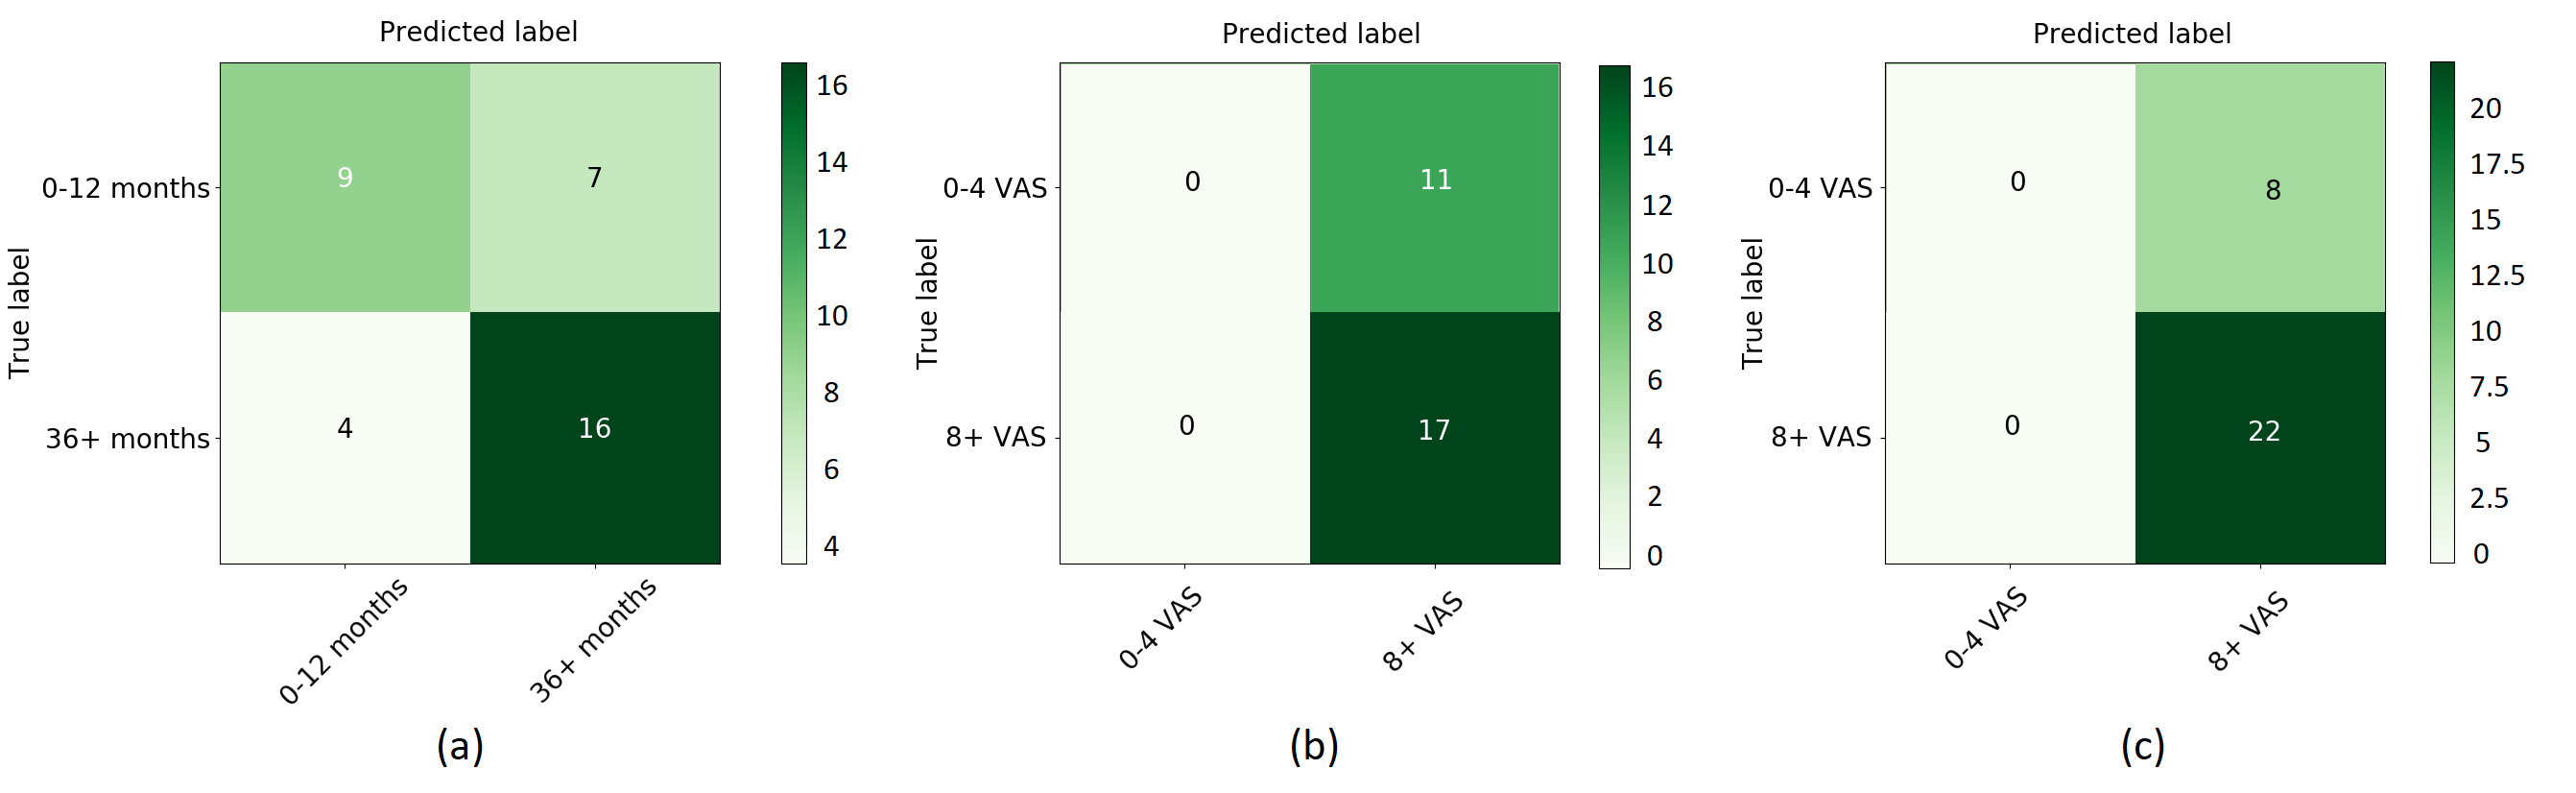
\includegraphics[width=1\textwidth]{Figures/samcon}
  \caption{Confusion matrices of (a) morphology-representation classified according pain duration, (b) location-representation classified according to pain intensity, and (c) combined-representation classified according to pain intensity.}
  \label{fig:confma}
\end{tcolorbox}
\end{figure*}

\subsection*{Optimization of the models}
During the optimization, a structured grid search resulted in different hyperparameters according to each model. This resulted in different optimizations in terms of the models with the morphology-representation. The learning rate was different according to pain duration (0.02), and pain intensity (0.1). A optimization in kernel initializer was defined as glorot\_uniform for pain duration, and glorot\_normal for pain intensity. The nodes was changed from 32 in the fully connected layers to 64 for pain duration, and 16 for pain intensity. Lastly, an optimization was found in number of epochs, and batch size, which was changed to 120 and 20 for pain duration, and 140 and 10 for pain intensity. The models including the location-representation had similar results from the optimization. A learning rate on 0.01, a glorot\_uniform kernel initializer, 16 nodes, and number of epochs and batch size on 120 and 20. 
Results of optimization on the combined-representation was almost identical for the two classifications. Both gave best performance with a glorot\_uniform kernel initializer, 16 nodes, and with a number of epochs and batch size of 120 and 30, to which the only difference was in the learning rate that for pain duration was 0.1, and 0.001 for pain intensity.

\subsection*{Performance of the models}
The average performance accuracy, sensitivity, and specificity of the models during test with new pain maps in different representations are shown in tab. \ref{tab:performance}. \newline
For the pain map representations that resulted in the highest accuracy for either pain duration or pain intensity, confusion matrices were created, and is shown in fig. \ref{fig:confma}.

%------------------------------------------------
\newpage
\section{Discussion}
This section discuss complexity of pain maps, and what may optimize the performance of the models. Furthermore, the results are discussed, whereas the highest performance value of the pain maps representations is evaluated. Finally, the performance according to the output, pain duration or pain intensity, is discussed.

\subsection*{Amount of pain maps}
A supervised deep learning model should use five thousand labeled data per category to obtain an acceptable performance \citep{Goodfellow2016}, whereas this study had a total number of pain maps (n=217) from uni- and bilateral PFP individuals. Based on the limited amount of pain maps, it was chosen to create more images by using a split body approach, where bilateral pain maps were split in two different pain maps. By using the split body approach and mirroring the pain to the right knee, it was assumed that pain duration and pain intensity were identical for both knees. Theoretically, the bilateral PFP may have occurred on one leg first, and afterwards have spreaded to the other knee, which could affect the pain duration. Furthermore, individuals with bilateral pain may feel more pain on one of the knees. This may have resulted in incorrected labeled pain maps, which could have an influence on the performance accuracy of the models.

\subsection*{Classification of pain maps}
The $R^2$-values of the linear correlations were close to zero represents nonlinearity, meaning that there are no simple correlation with the outputs, pain duration and pain intensity. Thus, a more complex model, such as deep learning model, is used to investigate the complexity of pain maps.
The deep learning models could classify both pain duration and pain intensity classes in the morphology-representation. Location-representation, despite of the given input, classified only according to the higher intervals (pain duration above 36 months and pain intensity above 8 VAS), and it could not classify according to the lower classes (pain duration below 12 month and pain intensity below 4 VAS). It can be observed in the confusion matrices of location-representation, where sensitivity of both inputs were equal to 0\% (thought of putting the image of conf matrix). Combined-representation, classified according to the pain duration, found the patterns in both classes, but overall accuracy was 55.56\%, which could be caused by including the knee regions as one of the features.
Based on the results, the accuracy of the representations containing the morphology, scored higher compared to location-representation. It can be discussed, that the morphology can be considered to be a better classification feature. Morphology scored 69.44\% and 60\% while location-representation scored 35.29\% and 60.71\%, reflecting pain duration and pain intensity.
Low score in location-representation is considered to be reflected as a result of imbalance between the duration intervals, as it could be also influenced with the deeper optimization. 
The low score could also be the result of the simplification of the location of the pain, that leads to the models not being able to find a pattern between the input and target output.  





\subsubsection*{Threshold } 
The location-representation had a 5\% threshold that defined when a pain region was considered active according to the amount of pain. It can be discussed whether this threshold was suitable, since adding the threshold resulted in loss of pain maps that had a very small amount of pain. However, a smaller threshold or no threshold would give active pain regions that might only contain very few pain pixels. Since PFP is described as hard to localize, it is unknown how precise the individuals have drawn their pain, thus every pixel should maybe not be taken into account. 
The combined-representation did not have a threshold for defining active pain regions, because the morphology of the pain would be affected when discarding small pain regions. 
This representation is thereby not a complete combination of the morphology- and location-representations. 

\subsection*{Classification according to output}
Generalization performance of the six models showed that pain duration was a more robust classifier compared to pain intensity. As a result, both classes of pain duration can be predicted in the morphology- and combined-representations, while classes representing pain intensity can be classified only with the morphology-representation.
It could be discussed that the lower results of pain intensity against the pain duration, is a reason of that, the pain intensity is a subjective statement and is considered as multifactorial, while pain duration is an objective parameter, and it is thereby expected that the models have a higher performance when classifying pain maps according to pain duration. 
Given the fact that the sensitivity for multiple models was 0\%, the accuracy becomes a reflection of the imbalance between classes in the test set, e.g. if the test subset contained 75\% of the class with high pain intensity, the accuracy would also be 75\%. This may also be a result of the relative small dataset used in this study.  
It is unknown whether the reason for the sensitivity to be 0\% is caused by that the models cannot find patterns according to the low valued pain intensity, or if it is a “fault” in the model that classifies all inputs as high pain intensity.  


\subsection*{Optimization of deep learning models}
Optimization of the models is often a time-consuming process based on the picks of the multiple hyperparameters and different algorithms which could be implemented during the development of the models.  
Activation functions were chosen based on the literature, where ReLU should be used for convolutional and fully connected layers in neural network models, and sigmoid should be picked for binary output layer. However, there was always a way for additional testing with softmax or linear activation function to increase the generalization performance. 
The dropout algorithm was set to the default 0.5 and used in all models between the fully connected layers to turn off the amount of nodes and prevent the models from overfitting. Additional values could have been tested in order to find most optimal for the every model.
Unfortunately, the lack of the time and time-consuming reruns during every optimization cycles, lead to use the most popular hyperparameters as there were many other which were tested with grid search 10-fold cross validation.
A further optimization of the models may be found according to the input parameters, to which more physical, and psychological features may increase the performance accuracy. Physical features, such as age, height, weight, physical activity niveau, and sport activity, may influence pain duration or pain intensity. Age could be a relevant feature since the perceived pain is dependent on the individual’s personality and character. Younger individuals may feel more pain because of a new and strange pain, than older individuals which have had PFP for a longer period of time. In addition older individuals may feel more pain because of the phenomenon central sentization, which in some cases result in widespread pain. The physical activity niveau, and sport may increase the pain intensity for some individuals because of the patellofemoral loaded activity. Psychological factors are an important feature to consider, because of its influence on pain intensity. Pain is multifactorial and can be influenced of psychosocial factors \citep{Roos2003}. Furthermore, other pain as hip pain may influence the PFP.
It may be considered to include either pain duration or pain intensity as an input to classify according to either pain intensity or pain duration, because of the possibility that there is a correlation between the two.
A limitation for this study was the available computational power for training of the model to which an improvement in performance may be found through more powerful systems or services.


%------------------------------------------------

\section{Conclusion}
conclusionnnnn

%----------------------------------------------------------------------------------------
%	REFERENCE LIST
%----------------------------------------------------------------------------------------

%\begin{thebibliography}{99} % Bibliography - this is intentionally simple in this template
%
%\bibitem[Figueredo and Wolf, 2009]{Figueredo:2009dg}
%Figueredo, A.~J. and Wolf, P. S.~A. (2009).
%\newblock Assortative pairing and life history strategy - a cross-cultural
%  study.
%\newblock {\em Human Nature}, 20:317--330.
% 
%\end{thebibliography}

%----------------------------------------------------------------------------------------
\begingroup
\raggedright

\bibliographystyle{unsrtnat}
\bibliography{bib}
%\urlstyle{same}
%
%
%\printbibliography
%\cleardoublepage

\endgroup
\end{document}